\documentclass{article}
\usepackage[T1]{fontenc}
\usepackage{lmodern}
\usepackage{graphicx}
\usepackage{amsmath,amssymb}
\usepackage[a4paper,margin=2cm]{geometry}
\usepackage[absolute,overlay]{textpos}
\setlength{\TPHorizModule}{1mm}
\setlength{\TPVertModule}{1mm}
\usepackage[indonesian]{babel}
\usepackage{hyperref}
\setlength{\emergencystretch}{2em}
% unit: Halaman 26

\begin{document}

% === Halaman 26 (llm) ===

Contoh:

\vspace{10mm}

\vspace{10mm}

\begin{align*}
(02 \bullet 26) \oplus (03 \bullet 7\text{B}) \oplus (01 \bullet \text{BD}) \oplus (01 \bullet 43) &= 3\text{F} \\
(01 \bullet 26) \oplus (02 \bullet 7\text{B}) \oplus (03 \bullet \text{BD}) \oplus (01 \bullet 43) &= 4\text{F} \\
(01 \bullet 26) \oplus (01 \bullet 7\text{B}) \oplus (02 \bullet \text{BD}) \oplus (03 \bullet 43) &= \text{F}9 \\
(03 \bullet 26) \oplus (01 \bullet 7\text{B}) \oplus (01 \bullet \text{BD}) \oplus (02 \bullet 43) &= 2\text{A}
\end{align*}

Semua perkalian dan penjumlahan dilakukan dalam $\text{GF}(2^8)$

Penjelasan tentang $\text{GF}(2^m)$ dapat dilihat pada lampiran

% deskripsi: Operasi perkalian matriks dalam field GF(2^8) yang menunjukkan perkalian matriks 4x4 dengan vektor kolom 4x1 menghasilkan vektor kolom 4x1.
% bbox normalisasi: [0.1700, 0.1200, 0.5400, 0.4100]
\begin{textblock*}{77.70mm}(35.70mm,35.64mm)
\noindent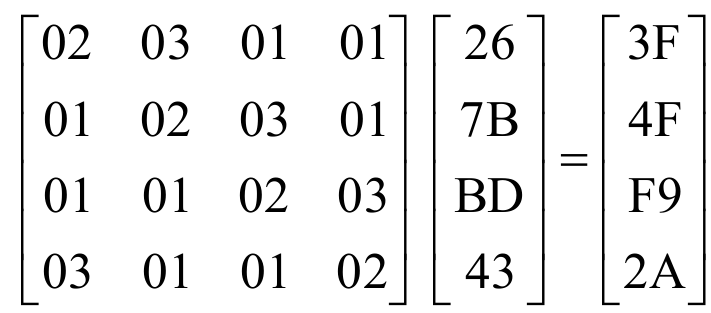
\includegraphics[width=77.70mm,height=86.13mm]{../../images/llm/page_026_img_01.png}%
\end{textblock*}

\end{document}
